\documentclass[twoside,a4paper]{article}
\usepackage{geometry}
\geometry{margin=1.5cm, vmargin={0pt,1cm}}
\setlength{\topmargin}{-1cm}
\setlength{\paperheight}{29.7cm}
\setlength{\textheight}{25.3cm}

% useful packages.
\usepackage{amsfonts}
\usepackage{amsmath}
\usepackage{amssymb}
\usepackage{amsthm}
\usepackage{enumerate}
\usepackage{graphicx}
\usepackage{multicol}
\usepackage{fancyhdr}
\usepackage{layout}

% some common command
\newcommand{\dif}{\mathrm{d}}
\newcommand{\avg}[1]{\left\langle #1 \right\rangle}
\newcommand{\difFrac}[2]{\frac{\dif #1}{\dif #2}}
\newcommand{\pdfFrac}[2]{\frac{\partial #1}{\partial #2}}
\newcommand{\OFL}{\mathrm{OFL}}
\newcommand{\UFL}{\mathrm{UFL}}
\newcommand{\fl}{\mathrm{fl}}
\newcommand{\op}{\odot}
\newcommand{\Eabs}{E_{\mathrm{abs}}}
\newcommand{\Erel}{E_{\mathrm{rel}}}

\begin{document}

\pagestyle{fancy}
\fancyhead{}
\lhead{Jovi Wong(3180104829)}
\chead{Math Software \#day1}
\rhead{2020/7/6}


\section*{I. Configure Environment}

\subsection*{I-a. Install Ipython} 

\begin{figure}[htp]
\centering
\includegraphics[width=4.5in]{ipython.jpeg}
\caption{Download from apt source}
\end{figure}
By the way, I have already installed python 3.6 before.
\vbox{}\vbox{}\vbox{}\vbox{}\vbox{}

\subsection*{I-b. Install Jupyter}
\begin{figure}[hbp]
\centering
\includegraphics[width=2.5in]{jupyter.jpeg}
\caption{Download from ubuntu software center}
\end{figure}
But I have some troubles on adding the kernel of octave into this editor, so I determine not to use it.
\vbox{}\vbox{}\vbox{}\vbox{}\vbox{}\vbox{}\vbox{}\vbox{}\vbox{}\vbox{}
\subsection*{I-c. Install Octave}
\begin{figure}[ht]
\centering
\includegraphics[width=4in]{octave.jpeg}
\caption{Download from ubuntu software center}
\end{figure}
\vbox{}\vbox{}\vbox{}\vbox{}\vbox{}
Then I install packages such as symbolic, image, optim and statistics via command line in Octave.

\section*{II. Problems and Examples}
\subsection*{Test Package Symbolic}
\large INPUT: x+3=3x \\
\large CODE: root = solve(x+3 == 3*x)\\
\large OUTPUT: root = $\frac{3}{2}$\\
\subsection*{Matrix Multiply}
\large INPUT: \\
a = [1 2 3]\\
b = [3 2 1]\\
\\
\large CODE: vm = a'*b\\
\\
\large OUTPUT: \\
vm =\\
     3 \qquad    2  \qquad   1\\
     6  \qquad   4 \qquad    2\\
     9 \qquad  6 \qquad    3\\
\subsection*{Vector Product}
\large INPUT: \\
a = [1 2 3]\\
b = [3 2 1]\\
\\
\large CODE \\
ip = dot(a,b) \\
op = cross(a,b)\\
\\
\large OUTPUT \\
ip = 10 \\
op = -4  \qquad   8  \qquad  -4 \\
\subsection*{Initialize Matrix}
\large INPUT \\
A = rand(3,3)\\
B = A(2:3, 1:2)\\
I = ones(4,4)\\
O = zeros(2,2)\\
\\
\large OUTPUT \\
A =\\
\qquad 0.868694705363510\qquad 0.431413827463545\qquad 0.136068558708664\\
\qquad 0.084435845510910\qquad 0.910647594429523\qquad 0.869292207640089\\
\qquad 0.399782649098896\qquad 0.181847028302852\qquad 0.579704587365570\\  
B =\\
\qquad 0.084435845510910\qquad 0.910647594429523\\
\qquad 0.399782649098896\qquad 0.181847028302852\\
I =\\
\qquad 1 \qquad 1 \qquad 1 \qquad 1\\
\qquad 1 \qquad 1 \qquad 1 \qquad 1\\
\qquad 1 \qquad 1 \qquad 1 \qquad 1\\
\qquad 1 \qquad 1 \qquad 1 \qquad 1\\
O =\\
\qquad 0\qquad 0\\
\qquad 0\qquad 0\\
\subsection*{Newton Iteration}
\large INPUT: f, df, err=1, $x_0=2$ \\
\\
\large CODE \\
iter = 0;\\
err = 1;\\
x0 = 2.0;\\
x = x0;\\
format long;\\
while(err $>$ 1e-8 and iter < 20)\\
x0 = x;\\
x = x0 - df(x0)/f(x0);\\
err = norm(x - x0);\\
iter = iter +1;\\
fprintf('iter \%d: x = \%18.15f, f(x) = \%28.15f', iter, x, f(x))\\
end\\
\\
\large OUTPUT \\
iter 1: x =  1.000000000000000, f(x) =            0.281718171540954 \\
iter 2: x =  0.914155281832543, f(x) =            0.012372566882760 \\
iter 3: x =  0.910017665783406, f(x) =            0.000030034837378\\ 
iter 4: x =  0.910007572548888, f(x) =            0.000000000179075\\ 
iter 5: x =  0.910007572488709, f(x) =            0.000000000000000 \\

\subsection*{Define Function and Plot}
\large INPUT: t = linspace(0,20,40); \\
\\
\large CODE \\
plot(t, besselj(0.5, t), 'r*-')\\
hold on\\
plot(t,besselj(1.5, t), 'b*--')\\
plot(t,besselj(5.5,t), 'cs-')\\
plot(t, besselj(10.5,t), 'mo--')\\
hold off\\
function y = myfunc(x)\\
$y = 3*x.^2 + 2*x + 18;$\\
end\\

function y = df(x)\\
    $y = 6*x -exp(x);$\\
end\\

function y = f(x)\\
    $y = 3*x.^2 - exp(x);$\\
end\\
\\
\large OUTPUT \\
\begin{figure}[bh]
\centering
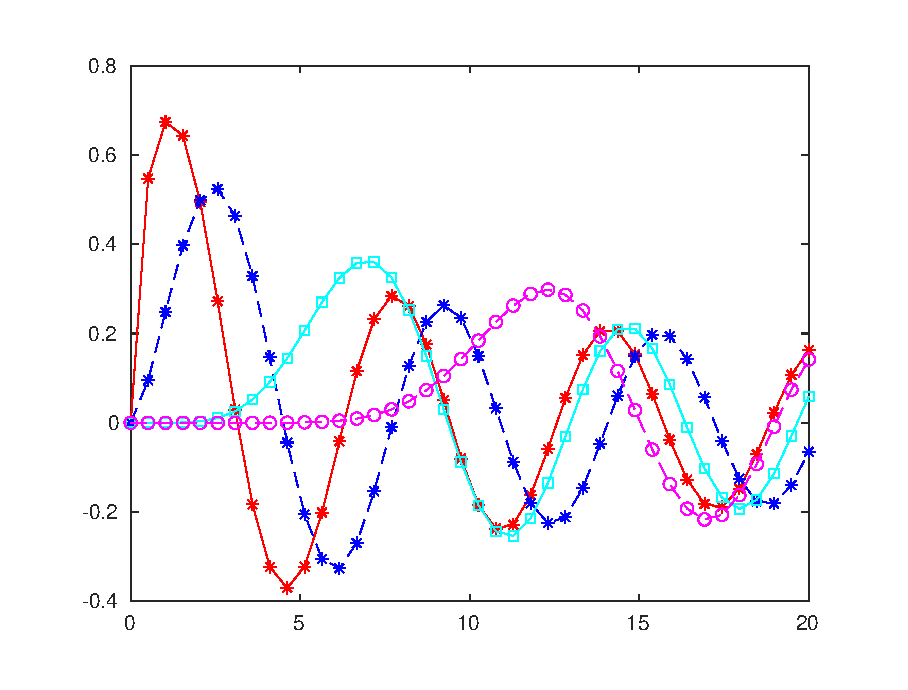
\includegraphics[width=2.1in]{Bessel.eps}
\caption{bessel fuction}
\end{figure}
\end{document}
%%% Local Variables: 
%%% mode: latex
%%% TeX-master: t
%%% End: 
